\documentclass[]{standalone}
\usepackage{tikz}
\usetikzlibrary{shapes,arrows,calc,positioning}
\usepackage{amsmath} % for dfrac
\usepackage{comment}
\usepackage{calc}

% definition of basic block
\tikzset{
    block/.style = {draw, rectangle,
        minimum height=1.2cm,
        minimum width=2cm},
    input/.style = {coordinate,node distance=1cm},
    output/.style = {coordinate,node distance=1cm},
    sum/.style = {draw, circle, node distance=1cm},
}

% definition of saturation block
\tikzset{% from https://tex.stackexchange.com/questions/161075/saturation-block
  saturation block/.style={%
    draw, 
    path picture={
      % Get the width and height of the path picture node
      \pgfpointdiff{\pgfpointanchor{path picture bounding box}{north east}}%
        {\pgfpointanchor{path picture bounding box}{south west}}
      \pgfgetlastxy\x\y
      % Scale the x and y vectors so that the range
      % -1 to 1 is slightly shorter than the size of the node
      \tikzset{x=\x*.4, y=\y*.4}
      %
      % Draw annotation
      \draw (-1,0) -- (1,0) (0,-1) -- (0,1); 
      \draw (-1,-.7) -- (-.6,-.7) -- (.6,.7) -- (1,.7);
    }
  }
}
\tikzset{% from https://tex.stackexchange.com/questions/161075/saturation-block
  deadband block/.style={%
    draw, 
    path picture={
      % Get the width and height of the path picture node
      \pgfpointdiff{\pgfpointanchor{path picture bounding box}{north east}}%
        {\pgfpointanchor{path picture bounding box}{south west}}
      \pgfgetlastxy\x\y
      % Scale the x and y vectors so that the range
      % -1 to 1 is slightly shorter than the size of the node
      \tikzset{x=\x*.4, y=\y*.4}
      %
      % Draw annotation
      \draw (-1,0) -- (1,0) (0,-1) -- (0,1);  % axis
      \draw (-1,1) -- (-.3,.3) -- (-.3,0) -- (.3,0) -- (.3,-.3) -- (1,-1);
	  %\draw (-.3,.3) -- (.3,-.3) ;
    }
  }
}

\begin{document}
	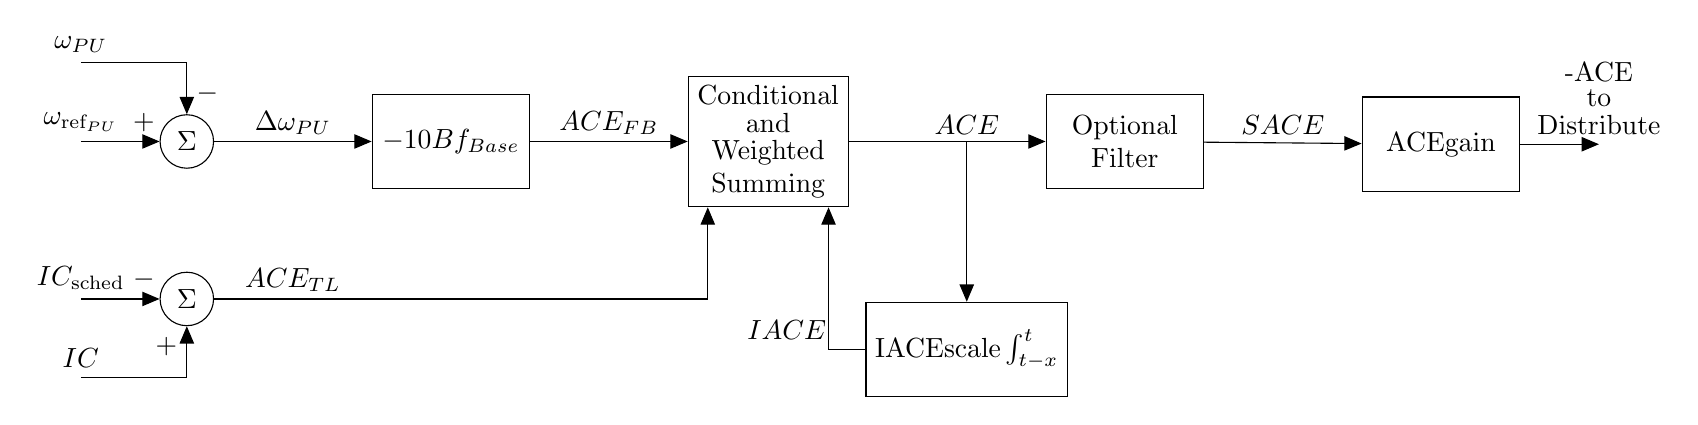
\begin{tikzpicture}[auto, node distance=1cm,>=triangle 45]
		% Starting inputwref
		\node [input, name=inputwref, label=$\omega_{\text{ref}_{PU}}$]  {};
		% Starting inputw
		\node [input, name=inputw, above=of inputwref, label=$\omega_{PU}$] (inputw) {};
		% sum 1
		\node [sum, right=of inputwref] (sum1) {$\Sigma$};
		% delta w node and label
		\coordinate [right=of sum1]  (deltaw) {};
		\coordinate [above=-.1em of deltaw,label={$\Delta\omega_{PU}$}]  (deltaWlabel){};
		
		% input ICsched
		\node [input, name=ICsched, below=2 cm of inputwref, label=$IC_{\text{sched}}$] {};
		% input IC
		\node [input, name=IC, below=of ICsched, label=$IC$] {};
		% sum 2
		\node [sum, right=of ICsched] (sum2) {$\Sigma$};
		% Tie Line ACE node and label
		\coordinate [right=of sum2]  (ACEtl) {};
		\coordinate [above=-.1em of ACEtl,label={$ACE_{TL}$}]  (ACEtllabel){};
		
		% Frequnecy Bias block
		\node [block, right=of deltaw] (fbias) {$-10Bf_{Base}$};
		% frequency Bias ACE node and label
		\coordinate [right=of fbias]  (ACEfb) {};
		\coordinate [above=-.1em of ACEfb,label={$ACE_{FB}$}]  (ACEfblabel){};
		
		% Conditional Summing
		\node [block, right=of ACEfb,] (condSum) {\shortstack{Conditional \\and \\Weighted\\ Summing}};
		%  ACE node and label
		\coordinate [right=1.5cm of condSum]  (ACE) {};
		\coordinate [above=-.1em of ACE,label={$ACE$}]  (ACElabel){};
		
		% Filtering
		\node [block, right=of ACE,] (filter) {\shortstack{Optional \\ Filter}};
		%  SACE node and label
		\coordinate [right=of filter]  (SACE) {};
		\coordinate [above=-.1em of SACE,label={$SACE$}]  (SACElabel){};
		
		% IACE
		\node [block, below=2 cm of ACElabel] (IACE) {$\text{IACEscale}\int_{t-x}^{t}$};
		\coordinate [left=1 cm of IACE,label={$IACE$}]  (IACElabel){};
		
		% output gain
		\node [block, right= of SACElabel] (ACE2dist) {$\text{ACEgain}$};
		% Pm out
		\node [output, right=of ACE2dist, label=$\shortstack{-ACE\\to\\Distribute}$] (output) {};
		
		% connecting lines
		\draw [draw,->] (inputwref) -- node[pos=0.8] {$+$} (sum1); 
		\draw [->] (inputw) -| node[pos=0.8] {$-$} (sum1);
		\draw [->] (sum1) -- (fbias);
		\draw [draw,->] (ICsched) -- node[pos=0.8] {$-$} (sum2); 
		\draw [->] (IC) -| node[pos=0.8] {$+$} (sum2);
		\draw [->] (fbias) -- (condSum);
		\draw [->] (sum2) -| ($(condSum.south west)!.25!(condSum.south)$); % using calc to find point halfway between corner and middle		
		\draw [->] (IACE) -| ($(condSum.south east)!.25!(condSum.south)$);
		\draw [->] ($(condSum)!.5!(filter)$) -| (IACE);
		%\draw [->] (ACElabel) -- (IACE);
		\draw [->] (condSum) -- (filter);
		\draw [->] (filter) -- (ACE2dist);
		\draw [->] (ACE2dist) -- (output);
		\begin{comment}
			
			\node [input, name=Pref, above= of sumP,label={[label distance=.1cm]0:$P_{\text{ref}}$} ] {};
			
			% Hz Deadband
			\node [deadband block, right=of deltaw, minimum size=3.5em,label=Hz deadband] (deadband) {};
			% delta w gain blocks
			\node [block, right=of deadband] (gain) {$\dfrac{M_{Base}}{R}$};
			\node [block, below=of gain] (Dt) {$M_{Base} Dt$};
			% Pref sum
			\node [sum, right=of gain] (sumP) {$\Sigma$};
			% limiter and labels
			\node [saturation block, right= of sumP , minimum size=3.5em, label=$MW_{cap}$] (mwcap){};
			\node [below=2em of mwcap, label=$0.0$](mwcapLOW){};
			% Valve state block
			\node [block, right=of mwcap] (state1) {$\dfrac{1}{1+\$T_s}$};
			
			% turbine state
			\node [block, right=of state1] (state2) {$\dfrac{1+\$T_3}{1+\$T_c}$};
			% Gov state
			\node [block, right=of state2] (state3) {$\dfrac{1+\$T_4}{1+\$T_5}$};
			% damping sum
			\node [sum, right= of state3] (sumd) {$\Sigma$};
			% Pm out
			\node [output, right=of sumd, label=$P_M$] (output) {};
			
			
			\draw [->] (Pref) -- node[pos=0.8] {$+$} (sumP);
			\draw [->] (sum1) -- (deadband) ;
			\draw [->] (deadband) -- (gain) ;
			\draw [->] (gain) -- (sumP) ;
			\draw [->] (sumP) -- (mwcap) ;
			\draw [->] (mwcap) -- (state1) ;
			\draw [->] (state1) -- (state2) ;
			\draw [->] (state2) -- (state3) ;
			\draw [->] (state3) -- node[pos=0.8] {$+$} (sum2);
			\draw [->] (deltaw) |-  (Dt); % line goes down and across
			\draw [->] (Dt) -|  node[pos=0.9] {$-$} (sumd); % line goes across then down
			\draw [->] (sumd) -- (output);
		\end{comment}
	\end{tikzpicture} 
\end{document}